% ------------------------------------------------------------------------
% file `main-bookexercise-3-exercise-body.tex'
%
%     exercise of type `bookexercise' with id `3'
%
% generated by the `exercise' environment of the
%   `xsim' package v0.21 (2022/02/12)
% from source `main' on 2026/10/10 on line 621
% ------------------------------------------------------------------------
1. 下图中，不属于\term{树}的结构是$\underline{\hspace{1cm}}$。\\
\begin{figure}[htbp]
    \centering
    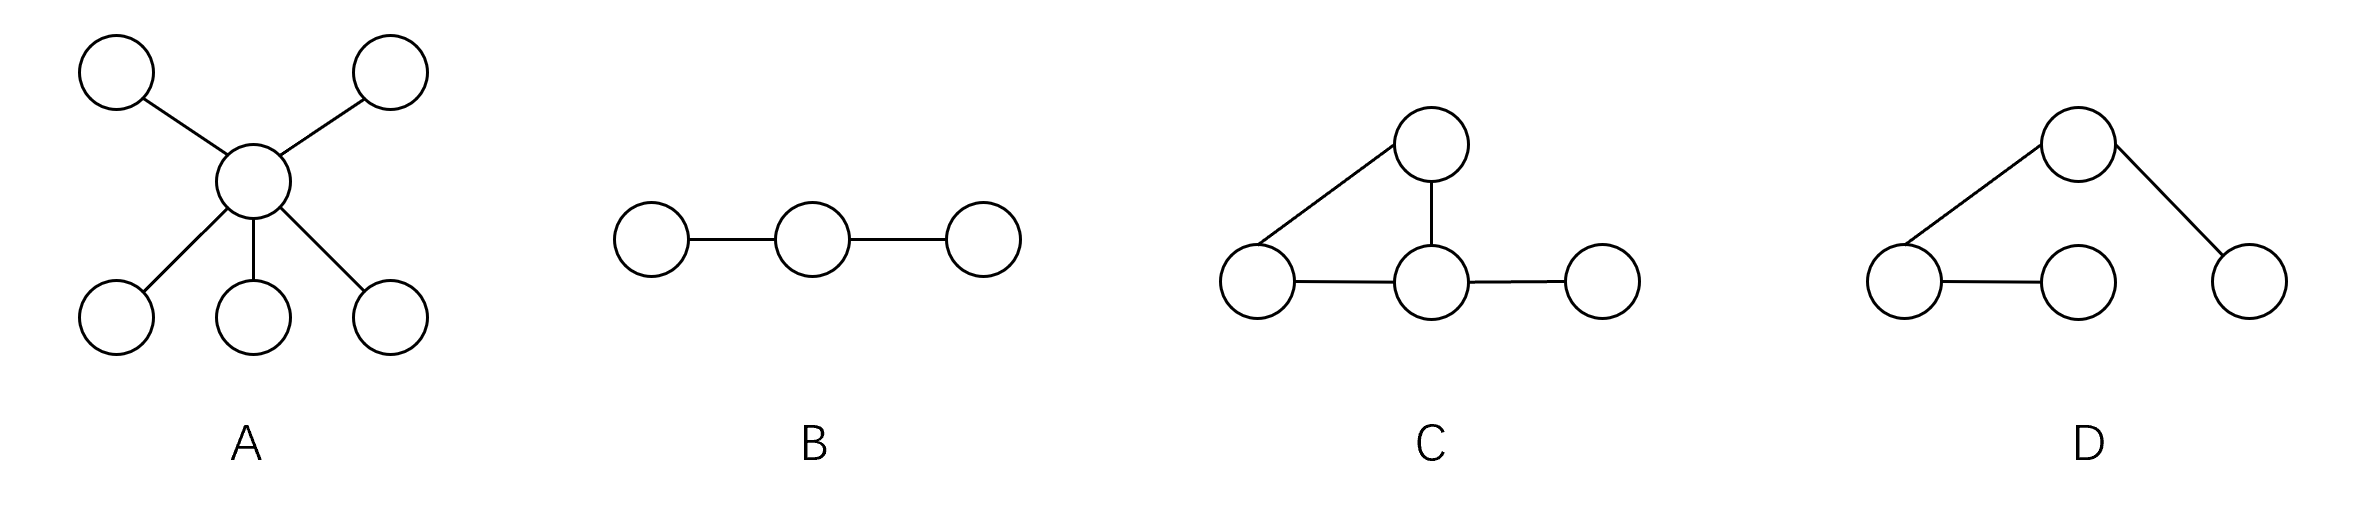
\includegraphics[width=0.75\textwidth]{assets/pics_and_ppts/ch4/下列结构中不是树的是.png}
    \caption*{}
    \label{fig:下列结构中不是树的是}
\end{figure}

2. 对于下图所示的树，下列说法错误的是$\underline{\hspace{1cm}}$。\\
\begin{figure}[htbp]
    \centering
    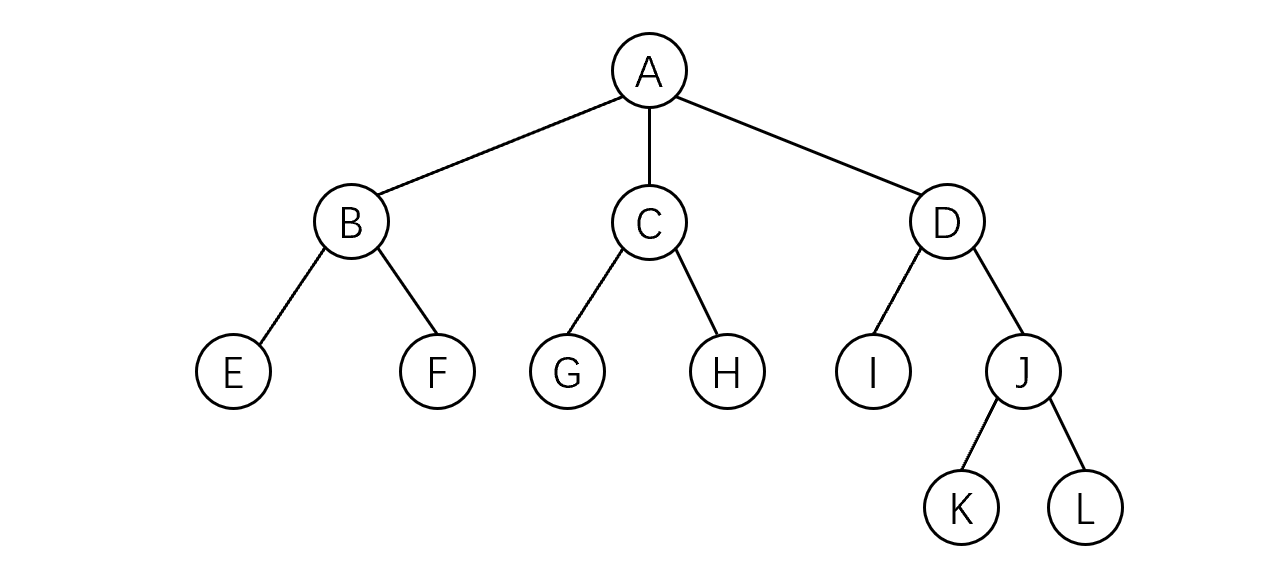
\includegraphics[width=0.55\textwidth]{assets/pics_and_ppts/ch4/考察树的基本概念的图.png}
    \caption*{}
    \label{}
\end{figure}

\noindent A. 节点B的度为2\\
B. 节点A的度为3\\
C. 这是一棵二叉树\\
D. 这棵树的度为3\\

3. 关于上题图所示的树，下列说法错误的是\\
A. 若根节点高度定义为1，则该树的高度为4\\
B. 若根节点高度定义为1，则该树的深度为3\\
C. 节点F的度为0，是叶子节点 \\
D. 以B、C、D为根节点的子树的集合构成了一个森林\\

4. 请观察下列四棵二叉树，分别统计每棵树中度为 0 的节点（叶节点）和度为 2 的节点的数量，并将结果填入表格。\\
\begin{figure}[htbp]
    \centering
    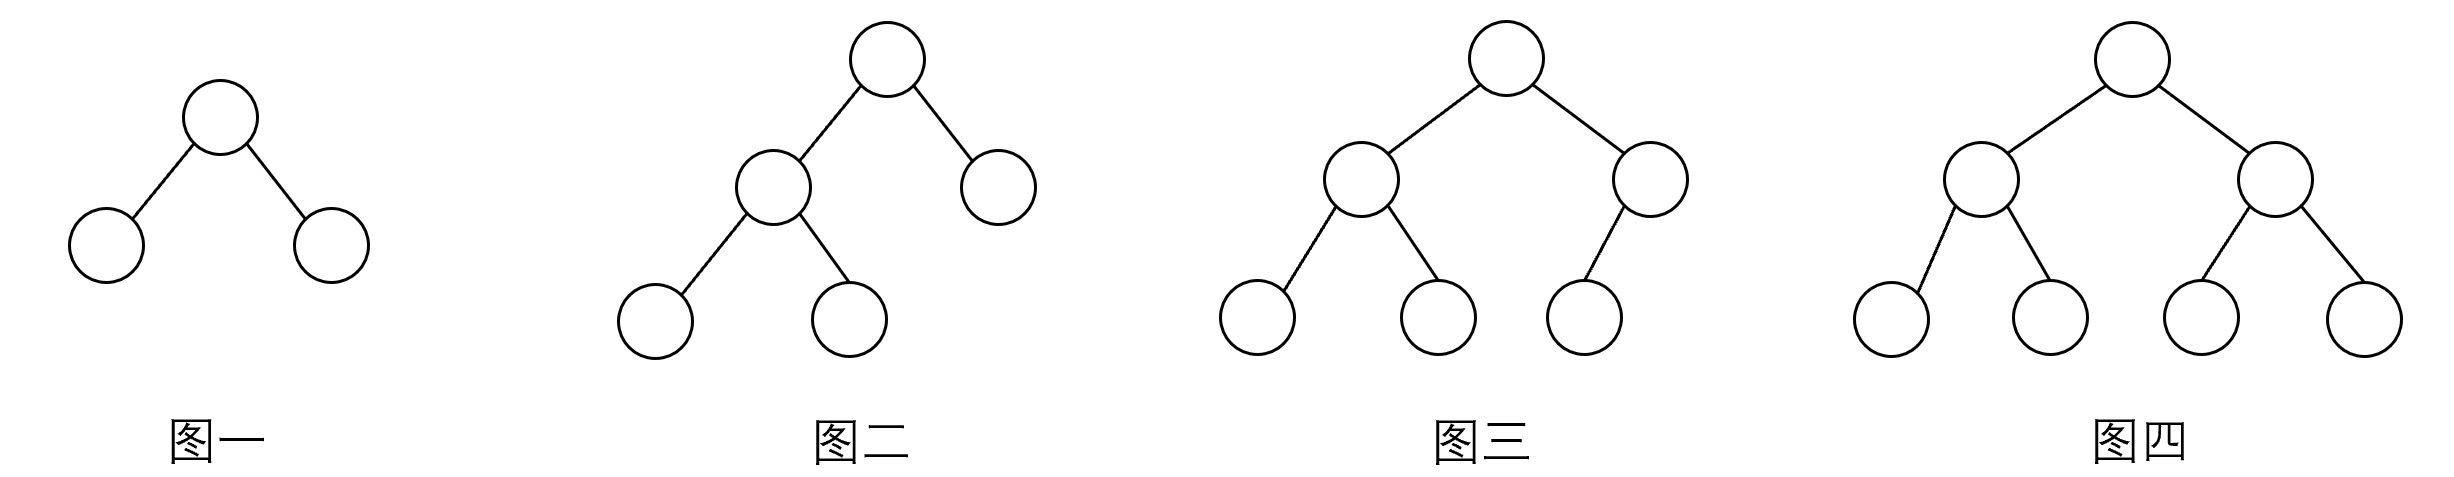
\includegraphics[width=0.95\textwidth]{assets/pics_and_ppts/ch4/习题图_推导n0n2关系.png}
    \caption*{}
    \label{fig:习题图_推导n0n2关系}
\end{figure}


\begin{center}
    \begin{tabular}{|c|c|c|}
        \hline
         & 度为 0 的节点数 & 度为 2 的节点数 \\
        \hline
        图一 &  &  \\
        \hline
        图二 &  &  \\
        \hline
        图三 &  &  \\
        \hline
        图四 & & \\
        \hline
    \end{tabular}
\end{center}

思考：
1）对于这四棵树，叶节点数与度为 2 的节点数之间有什么关系？\\[0.5em]
2）这种关系是否可能对任何非空二叉树都成立？请尝试画出其他形状的二叉树，检验你的猜想。\\[0.5em]
3）不必从数学角度严谨证明，你能否尝试解释，为什么这两个数量之间会存在这样的关系？\\[0.5em]


5. 一棵非空二叉树中，有 8 个度为 2 的节点，3 个度为 1 的节点。请问：\\
1）能否确定这棵二叉树有多少个叶节点？\\[0.5em]
2）能否确定这棵二叉树一共有多少个节点？\\[0.5em]

6. 一棵非空二叉树共有 20 个节点，其中有 7 个度为 1 的节点。请问这棵二叉树的叶节点数可能是多少？\\

7. 下图中，是满二叉树的有$\underline{\hspace{1.7cm}}$；不是满二叉树，但是是完全二叉树的有\underline{\hspace{1.7cm}}。
\begin{figure}[htbp]
    \centering
    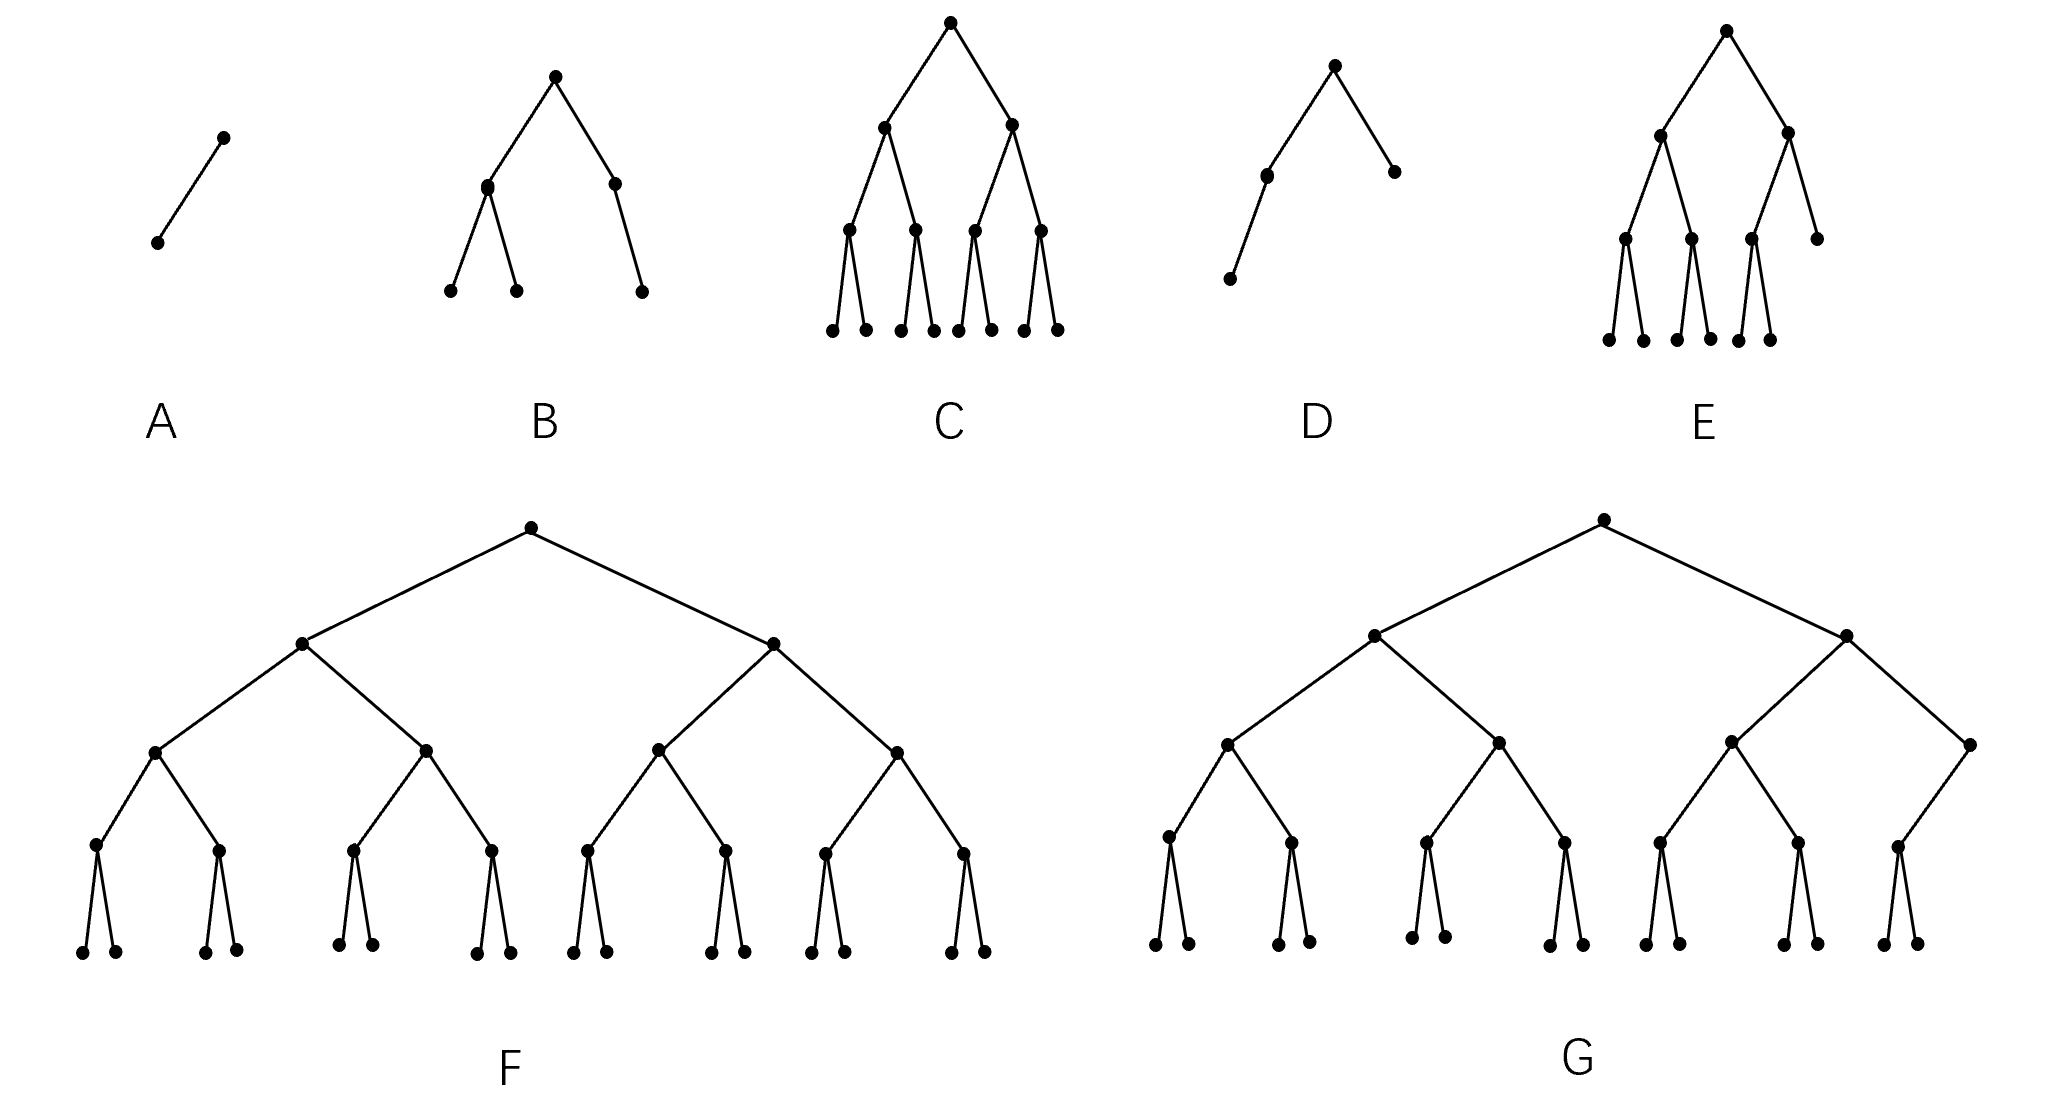
\includegraphics[width=1.03\textwidth]{assets/pics_and_ppts/ch4/习题图_判断满二叉树与完全二叉树.png}
    \caption*{}
    \label{fig:习题图_判断满二叉树与完全二叉树}
\end{figure}

8. [多选]若完全二叉树有n（n > 0）个节点，从上到下，从左到右分别编号1至n，则下列说法中正确的有\underline{\hspace{1cm}}\\[0.5em]
A. 若某节点不是根节点，其编号为i，则其父节点的编号为$ \left\lfloor \frac{i}{2} \right\rfloor $ \\
B. 若某节点编号为i，且 2 * i > n，则节点 i 一定是叶子节点\\
C. 树中度为1的节点数可能大于1\\
D. $\left\lfloor \frac{n}{2} \right\rfloor $一定是所有非叶子节点中，编号最大的那个\\


